\documentclass{article}

% Packages
\usepackage[utf8]{inputenc}
\usepackage[T1]{fontenc}
\usepackage{lipsum} % For dummy text
\usepackage{physics} % For physics notation
\usepackage{amsmath} % For math
\usepackage{amssymb} % For math symbols 
\usepackage[margin=2cm]{geometry} % For smaller margins
\usepackage{gensymb} % For degree symbol
\usepackage{diagbox} % For table
\usepackage{slashbox} % For table
% \usepackage[margin=1in,headheight=57pt,headsep=0.1in]{geometry}
\usepackage{hyperref}
\usepackage{xcolor} % for colored text
\usepackage{graphicx} % For \includegraphics
\usepackage{float}    % For the [H] placement specifier
\usepackage{biblatex} %Imports biblatex package
\addbibresource{sample.bib} %Import the bibliography file

% Document information
\title{FYP Report}
\author{Lin Zhonglin}
\date{\today}
\usepackage{setspace}
% Using \doublespacing in the preamble 
% changes the text to double-line spacing
\doublespacing
\begin{document}
\noindent

\maketitle
\tableofcontents

\section{Overview}
\begin{enumerate}
    \item Background: 
    \item Key part of my work: (depends on how far I go)
        \begin{enumerate}
            \item The optimised pulse for a particular state preparation
            \item how it differs from other pulse (Chiyuan's alternate pulse way)
            \item Go from model Hamiltonian to physical Hamiltonain, 
                    discuss the approximations' effect, 
                    compare fideilty
        \end{enumerate}
\end{enumerate}

TODO: 
\begin{enumerate}
    \item Go through the Hamiltonian derivation 
            $\rightarrow$ for comparison of fidelity later 
    \item does Qutip considers the cavity Hilbert space truncation discussed below? 
\end{enumerate}


Issues to be dealt with: 
\begin{enumerate}
    \item local minima / maxima in optimization algorithm
    \item Reinhold: 
        Optimizing a full unitary operation is sensible for qubits, or systems of a few qubits, but in the cavity manipulations to be performed in the following sections, this is not usually a sensible operation, since doing operations involving states at the border of the truncation (i.e. the maximum photon number state considered in the simulation), would typically require a larger truncation to simulate accurately (driving $\ket{n_{ph}}$) will almost always in part bring us partially to $\ket{n_{ph} + 1}$.
\end{enumerate}


%%%%%%%%%%%%%%%%%%%%%%%%%%%%%%%%%%%%%%%%%%%%%%%%%%%%%%%%%%%%%%%
\section{Background, theory and motivation}
%%%%%% 草稿 %%%%%%%%
content: 
introduce the idea of bosonic-modes-encoded qubits, give a simple example;
motivate Bosonic-modes-encoded qubits 
    -> that one physical device now can encode multiple qubits
    -> this also makes error correction more efficient -> easier to control multiple qubits

introduce cavity-transmon system 
motivate for cavity-DQD system

theory of cavity-DQD: 
original Hamiltonians -> rotation, approximaition, dispersive regime, etc... -> the Hamiltonian I used for pulse optimization

briefly bridge to and cover the overview of content of this report: 
1. basic theory on optimization, QuTip, GRAPE, CRAB, etc...
2. pulse optimization for state preparation
3. compare fidelity from approximate Hamiltonian with fidelity from original Hamiltonian 
4. possible future work: gate design, model noise
%%%%%% 草稿 %%%%%%%%

Quantum computing has emerged as a paradigm with the potential to solve problems that are intractable for classical computers. Among the various physical implementations of qubits, the cavity-coupled transmon system has become a leading platform due to its strong nonlinearity and large Hilbert space. This system leverages the coupling between the transmon qubit and the cavity to achieve robust qubit control and readout \cite{blais2004, houck2008}.

One of the key advantages of using a cavity for quantum computing is its potential for quantum error correction. By encoding a single logical qubit into multiple cavity Fock states, it is possible to protect against certain types of errors, thus enhancing the reliability of quantum computations \cite{girvin2014, ofek2016}.

Despite the success of the cavity-coupled transmon system, there is ongoing research into alternative qubit implementations that may offer further advantages. One such alternative is the cavity-coupled Double Quantum Dot (DQD) system. This system combines the advantages of semiconductor quantum dots, such as scalability and compatibility with existing semiconductor technology, with the strong coupling and large Hilbert space provided by the cavity. The DQD system has the potential to achieve high-fidelity qubit operations while maintaining the error correction capabilities of cavity-based systems \cite{petersson2012, mi2018}.

The control and manipulation of quantum systems are central to the realization of quantum computing. Quantum optimal control theory provides a framework for designing control protocols that achieve desired quantum operations with high fidelity. In this context, the goal is to find optimal control fields that drive the evolution of the quantum system from an initial state to a target state or implement a specific unitary transformation. Techniques such as Gradient Ascent Pulse Engineering (GRAPE) and Chopped Random Basis (CRAB) optimization are commonly used to find these optimal control fields \cite{khaneja2005, cai2011}. These methods involve numerically optimizing a cost function, typically related to the fidelity between the achieved and desired quantum states, subject to constraints imposed by the physical system and control hardware.

In this report, we explore the application of quantum optimal control theory to the cavity-coupled DQD system for state preparation tasks. We compare the performance of different control optimization algorithms and investigate the effects of various approximations and constraints on the control fidelity. Through this study, we aim to demonstrate the potential of the cavity-coupled DQD system as a platform for quantum computing and contribute to the development of robust control techniques for quantum technologies.

%%%%%%%%%%%%%%%%%%%%%%%%%%%%%%%

%%%%%%%%%%%%%%%%%%%%%%%%%%%%%%%%%%%%%%%%%%%%%%%%%%%%%%%%%%%%%%%
\subsection{Hamiltonians of physical system}
% discuss 
% - Full Original Hamiltonian 
% - effective Hamiltonian (same as )

\subsection{Quantum Optimal control}
We assume we have a quantum system, whose Hamiltonian can be written in the following form: 

\begin{figure}[H]
    \centering
    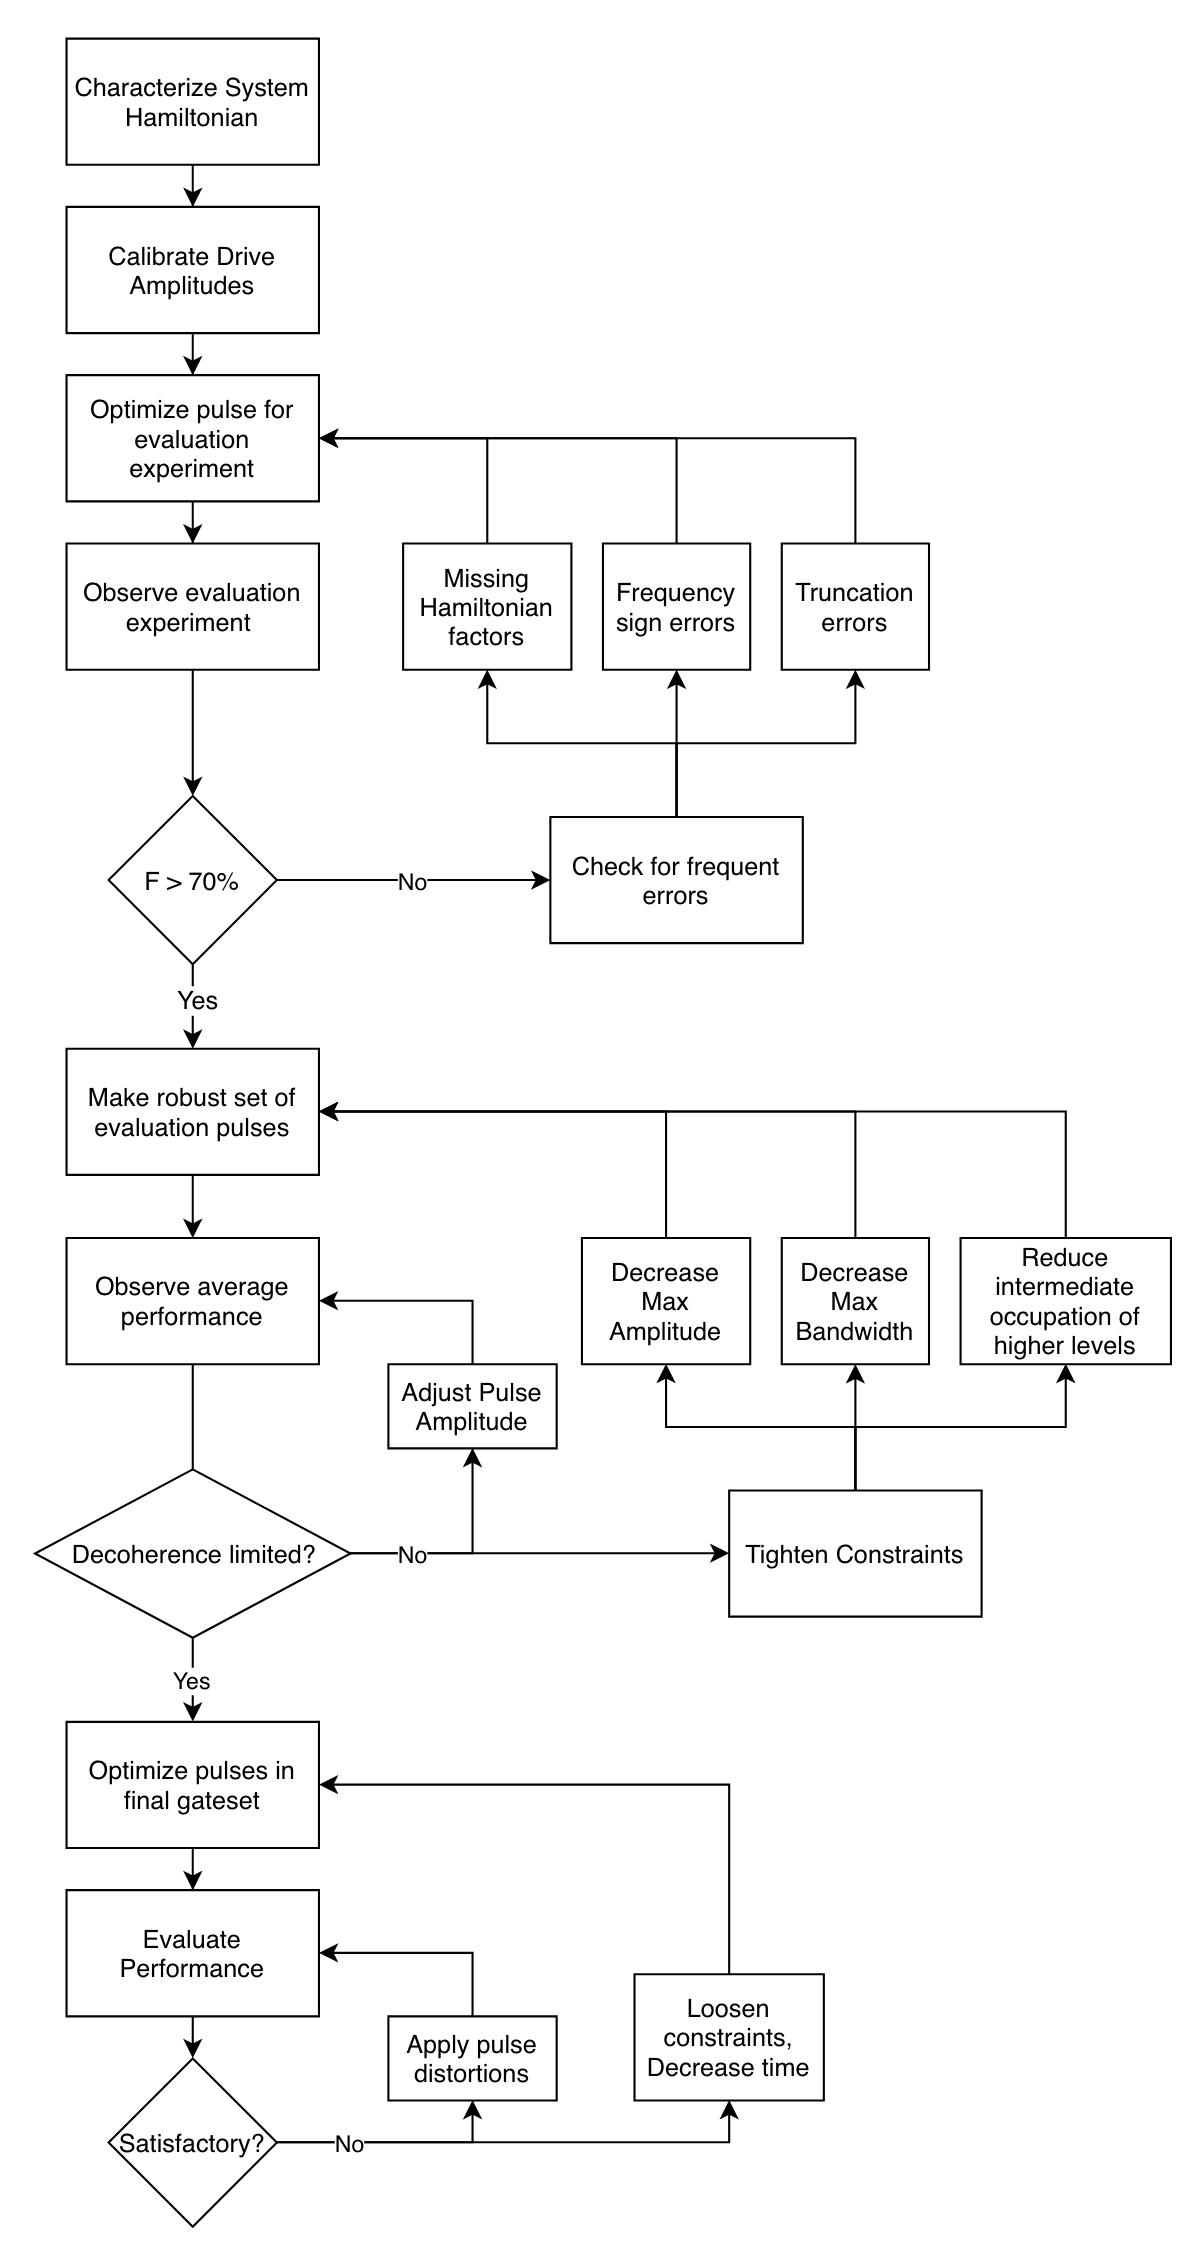
\includegraphics[width=0.6\linewidth]{flowchart.png}
    \caption{Flowchart for optimal control system}
    \label{fig:flowchart}
\end{figure}

Overview of Quantum Optimal Control
Quantum optimal control theory is a cornerstone of quantum technology, providing a systematic approach to manipulate quantum systems with high precision. The theory aims to determine the control strategies that steer a quantum system from an initial state to a desired final state with maximum efficiency. This is crucial for the development and implementation of quantum computing, quantum sensing, and quantum communication technologies. The central challenge in quantum optimal control is to optimize control parameters, such as pulse shapes or sequences, to achieve high-fidelity quantum operations while minimizing errors and resource consumption \cite{glaser2015, brif2010}.

Basic Types of Quantum Optical Control
Within the realm of quantum control, quantum optical control stands out as a key approach for manipulating quantum systems using electromagnetic fields. Coherent control and feedback control are two primary types in this domain. Coherent control involves shaping and timing electromagnetic fields to drive the quantum system's evolution coherently. This method is widely employed in controlling atomic and molecular systems, quantum dots, and superconducting qubits \cite{shapiro2012, chow2010}. On the other hand, feedback control involves measuring the quantum system and using the outcomes to adjust the control fields in real-time, which is essential for error correction and stabilization in quantum systems \cite{wiseman2009}.

Overview and Basic Types of Quantum Pulse Optimization
Quantum pulse optimization is a critical aspect of quantum control, focusing on finding the optimal control pulses for driving a quantum system's evolution. GRAPE, CRAB, and Krotov's methods are three widely used techniques in this area. GRAPE optimizes control pulses by numerically calculating the gradient of a fidelity measure concerning the control parameters. It is particularly effective for systems with a large number of control parameters \cite{khaneja2005}. CRAB, on the other hand, reduces the complexity of the optimization problem by expanding the control pulses in a random basis and optimizing the expansion coefficients \cite{doria2011}. Krotov's method is known for its monotonic convergence, making it suitable for problems where this property is crucial, such as open quantum systems \cite{reich2012}.

Python Packages for Quantum Optimal Control
To facilitate quantum control simulations and optimizations, several Python packages have been developed. QuTiP is a comprehensive framework for simulating the dynamics of open quantum systems and includes tools for quantum control optimization \cite{johansson2013}. The Krotov package, built on top of QuTiP, specifically implements Krotov's method for quantum optimal control, providing a user-friendly interface for solving quantum control problems \cite{goerz2019}.



%%%%%%%%%%%%%%%%%%%%%%%%%%%%%%%
\subsection{Figure of merit, cost function}
state transfer case
single-state state transfer: 
\begin{align*}
    f(\vec{\epsilon}(t)) &= \mathcal{F}(\vec{\epsilon}(t)) \quad \text{state fidelity}\\
    &\equiv \abs{\bra{\psi_{targ}} U(T,\vec{\epsilon}(t)) \ket{\psi_{init}}}^2 \\
    &= \abs{\bra{\psi_{targ}} 
        \mathcal{T}\exp{-\frac{i}{\hbar}\int_0^T dt H(\vec{\epsilon}(t))}
        \ket{\psi_{init}}}^2 \\
    &\text{make the problem numerical, make $\vec{\epsilon}(t)$ a piece-wise constant function with $N=T/\delta t$,} \\
    &\text{$\delta t$ is a parameter, usually set to time resolution of AWG.} \\
    &= \abs{\bra{\psi_{targ}} 
        U_NU_{N-1}...U_1
        \ket{\psi_{init}}}^2, \quad \text{where, } U_k=\exp{\frac{i\delta t}{\hbar}H(\vec{\epsilon}(k\delta t))} \\
\end{align*}

multi-state state transfer:
\begin{align*}
    f(\vec{\epsilon}(t)) &= \mathcal{F}(\vec{\epsilon}(t)) \quad \text{Fidelity}\\
    &\equiv 
        \begin{cases}
            \abs{\sum_k \bra{\psi_{targ}^{(k)}} U(T,\vec{\epsilon}(t)) \ket{\psi_{init}^{(k)}}}^2 &\text{coherent} \\
            \sum_k \abs{\bra{\psi_{targ}^{(k)}} U(T,\vec{\epsilon}(t)) \ket{\psi_{init}^{(k)}}}^2 &\text{inoherent}
        \end{cases} \\
    &\text{for coherent case with number of state = dimension of Hilbert space,}\\
    &=\abs{\text{Tr}\left[U(T,\vec{\epsilon}(t))U_{targ}^{\dagger}\right]}^2 \quad \text{unitary fidelity}\\
\end{align*}

open system case: 

%%%%%%%%%%%%%%%%%%%%%%%%%%%%%%%
\subsection{Pulse constraints}
\begin{enumerate}
    \item constraints come from AWG(Arbitrary Wave Generator)'s amplitude and bandwidth constraints
        $\rightarrow$ consider adding a set of constraint terms to the cost function
        \begin{equation*}
            f(\vec{\epsilon}(t)) = \mathcal{F}(\vec{\epsilon}(t)) + \sum_i \lambda_i g_i(\vec{\epsilon})
        \end{equation*}
    \item pulse amplitude: the output power of our AWG is limited, and thus to be feasible, we need $\epsilon(t) ≤ \epsilon_{max}$ for all t. $\rightarrow$ hard cutoff / soft cutoff
        \begin{enumerate}
            \item Employ an optimization algorithm which naturally allows for such constraints $\rightarrow$ see K-BFGS-B in scipy.optimize
            \item Parametrise optimization problen 
                \begin{align*}
                    &\stackrel{\text{maximize}}{\vec{\epsilon}(t)}  \mathcal{F} (\vec{\epsilon}(t)) 
                    \rightarrow \stackrel{\text{maximize}}{\vec{x}}  \mathcal{F} (\vec{\epsilon}(\vec{x})) \\
                    &\text{where, } \epsilon_k = \epsilon_{max} \tanh{(x_k)} 
                \end{align*}
        \end{enumerate}
    \item pulse bandwidth:   
        \begin{itemize}
            \item soft cutoff
            \item hard cutoff
            \item linear frequency-dependent penalty
        \end{itemize}
\end{enumerate}

\subsubsection{limit the intermediate photon number}
Since computer memory is finite, we are forced to choose a photon number truncation nph such that the operator a becomes a $n_{ph} \times n_{ph}$ matrix. 
When we do this, we are in effect replacing our infinite-dimensional oscillator with a finite-dimensional qudit. 
This replacement is only valid if all of the system dynamics relevant for the desired state transfers occurs within the $\{\ket{0} ,\cdots , \ket{n_{ph} - 1} \}$ subspace. 
For generic applied drives this is not the case. In order to enforce this property, we modify the optimization problem to find a solution which operates identically under several different values of $n_{ph}$.
Writing the fidelity as computed with a truncation nph as $F_{n_{ph}}$, we have:
\begin{equation}
    \stackrel{\text{maximize}}{\vec{\epsilon}} \left( \sum_k F_{n_{ph}+k} (\epsilon(t)) \right) - \left( \sum_i \lambda_i g_i (\epsilon(t)) \right)
\end{equation}

\begin{itemize}
    \item To enforce that the behavior is identical in the different truncations, we add the penalty term: 
        \begin{equation*}
            g_{\text {discrepancy }}(\boldsymbol{\epsilon}(\boldsymbol{t}))=\sum_{k_1 \neq k_2}\left(\mathcal{F}_{n_{\mathrm{ph}}+k_1}(\boldsymbol{\epsilon}(t))-\mathcal{F}_{n_{\mathrm{ph}}+k_2}(\boldsymbol{\epsilon}(t))\right)^2
        \end{equation*}
        I think it's making the cost function symmetrical w.r.t. $n_{ph}$.
    \item A more recently developed, and more direct, method is to add a penalty term for any occupation of the final photon state ($\ket{n_{ph} - 1}$) in the truncated Hilbert space at any time:
        \begin{equation*}
            g_{\text {trajectory }}=\sum_{k=1}^N\left|\left\langle n_{\text {ph }}-1 \mid \psi_{\text {fwd }}^{(k)}\right\rangle\right|^2
        \end{equation*}
        Not sure what this is doing, putting here for possible future use. 
\end{itemize}

\textcolor{red}{Not sure whether this is implemented in QuTip.}

\subsubsection{Troubleshooting optimization convergence}
Possible issue: 
\begin{itemize}
    \item 
\end{itemize}

Check list: 
\begin{enumerate}
    \item Check that the time given $T = N \delta t$ is appropriate.
        \begin{itemize}
            \item Specified in units that are consistent with the units specifying the Hamiltonian. For instance, if the Hamiltonian is specified in GHz, then the time step should be in units of ns.
            \item N value appropriate
        \end{itemize}
    \item check constraints
        \begin{itemize}
            \item Completely remove all constraints and penalties, and make sure that the algorithm works in this context before re-introducing them
        \end{itemize}
    \item check algorithm 
        \begin{itemize}
            \item check termination conditions \\
            Gradient based search algorithms usually have termination conditions specified in terms of the norm of the gradient. It is often necessary to lower the gradient norm threshold for termination to ensure that it does not give up -> gtol in scipy.minimize

        \end{itemize}
    \item check ionitial guess
        \begin{itemize}
            \item Avoid special initial guesses, this depends on the algorithm. 
                For gradient-based algo, make sure initial gradient is not vanishing.
        \end{itemize}
    \item miscellaneous checks
        \begin{itemize}
            \item Truncation of cavity-state Hilbert space large enough? 
        \end{itemize}
\end{enumerate}

%%%%%%%%%%%%%%%%%%%%%%%%%%%%%%%
\subsection{Pulse optimization algorithms}
\begin{itemize}
    \item Quantum control
        \begin{itemize}
            \item prepare some specific state
            \item effect some state-to-state transfer
            \item effect some transformation (or gate) on a quantum system
        \end{itemize} 
\end{itemize}

%%%%%%%%%%%%%%%%%%%%%%%%%%%%%%%
\subsubsection{GRAPE: Gradient Ascent Pulse Engineering}
GRAPE algorithm in QuTip: 
\begin{enumerate}
    \item overview: \\
    \begin{itemize}
        \item The combined Hamiltonian is approximated as: $H(t) \approx H\left(t_k\right)=H_0+\sum_{j=1}^M u_{j k} H_j$ \\
        where,  k is a timeslot index, 
                j is the control index, 
                and M is the number of controls. 
                Hence $t_k$ is the evolution time at the start of the timeslot, 
                and $u_{jk}$ is the amplitude of control j throughout timeslot k.
                Number of time steps $N=T/\delta t$.\\
        \item The time evolution operator, or propagator, within the timeslot can then be calculated as:  
                $U_k:=e^{-i H\left(t_k\right) \Delta t_k}$ \\
                where, $\Delta t_k$ is the duration of the timeslot.\\
                The evolution up to (and including) any timeslot k (including the full evolution k=M) can the be calculated as 
                $U\left(t_k\right):=U_k U_{k-1} \cdots U_1 U_0$
        \item figure of merit: See Reinhold thesis section
        \item optimization algorithm: 
            \begin{enumerate}
                \item There are now $N\times M$ variables to minimize the figure of merit. 
                    The problem becomes a \underline{finite multi-variable optimization problem}.
                \item Optimization algorithm: (see Reinhold thesis section for details)\\
                    Gradient and quasi-Newton method (considers Hessian) both implemented.\\
                    (The default method in the QuTiP Qtrl GRAPE implementation is the L-BFGS-B method in Scipy)
                \item calculating / approximating the gradient: see Reinhold thesis section

            \end{enumerate}
    \end{itemize}
\end{enumerate}

\begin{equation}
    H(\vec{\epsilon}(t)) = H_0 + \sum_{k=1}^m \epsilon_k(t) H_k
\end{equation}
Goal: Find optimal control field $\vec{\epsilon}(t)$ that optimizes some function $f(\vec{\epsilon}(t)) = f(H(\vec{\epsilon}(t)))$. \\
\begin{enumerate}
    \item To optimize a large number of parameters, we need:
        \begin{enumerate}
            \item an efficient means of calculating the gradients of cost function w.r.t parameters
            \item sub-optial local minima are sufficiently unlikely or close to global minima
        \end{enumerate}
    \item Given methods to calculate cost function and gradients, we have two main classes of algorithm for performing optimization: 
        \begin{itemize}
            \item line-search methods: one alternates between picking a direction in parameter space, radiating from our current point, and subsequently performing a 1-d minimization protocol to find the minimum along this line. \\
                $\rightarrow$ basic gradient descent: choose direction as gradient at the point. \\
                $\rightarrow$ Newton method: choose direction using both gradient and Hessian matrix at the point. $\rightarrow$ quasi-Newton, L-BFGS
            \item trust-region methods
        \end{itemize}
    \item calcualte gradient of $f(\vec{\epsilon}(t))$ with respect to $\vec{\epsilon}(t)$
        \begin{enumerate}
            \item For an analytical function $f(\vec{\epsilon})$, gradient is given by $\nabla f(\vec{\epsilon}) = \sum_{i=1}^m \frac{\partial f(\vec{\epsilon})}{\partial \epsilon_i} \hat{\epsilon}_i$
            \item For discrete $\vec{\epsilon}$, gradient of $f(\vec{\epsilon})$ is given by the finite difference method.
            \item approximate the gradient: skipping here.
            \item When calculating / approximating gradient is too expensive, cosider optimization algorithm other than gradient descent.
        \end{enumerate}
    \item take a step (step size as a parameter) in the direction. \\
        step size too small: optimization takes long\\
        step size too large: may never reach true optima
    \item calcualte gradient again
    \item repeat until convergence
    \item issue of local minima / maxima: 
        \begin{itemize}
            \item Optimize for infidelity (1 - fidelity) instead of fidelity. 
                Because infidelity is lower bounded by 0. Terminate optimization when infidelity reaches 0 or close to 0. 
        \end{itemize}
\end{enumerate}

%%%%%%%%%%%%%%%%%%%%%%%%%%%%%%%
\subsubsection{CRAB: Chopped RAndom Basis}
CRAB-Chopped RAdom Basis algorithm in QuTip: 
\begin{enumerate}
    \item rough overview: 
    \item Since the pulse complexity is usually very low, it is sufficient to transform the optimal control problem to a few parameter search by introducing a physically motivated function basis that builds up the pulse. 
        Compared to the number of time slices needed to accurately simulate quantum dynamics (often equals basis dimension for Gradient based algorithms), this number is lower by orders of magnitude, 
        allowing CRAB to efficiently optimize smooth pulses with realistic experimental constraints. 
    \item choosing functional basis: 
        \begin{itemize}
            \item Consider a priori knowledge of the system \\
                $\rightarrow$ such as symmetries, magnitudes of scales,... \\
                $\rightarrow$ integrate experimental constraints such as maximum frequencies allowed, maximum amplitude, smooth ramping up and down of the pulse ...
            \item Consider expected solution (e.g. sign, smoothness, bang-bang behavior, singularities, maximum excursion or rate of change,....).
        \end{itemize}
    \item where CRAB differs from GRAPE: 
        \begin{itemize}
            \item Optimized pulse from CRAB is a smooth function.
            \item CRAB optimizes pulse function basis coefficient instead of amplitude of poulse at time slices.
            \item CRAB considers time slices only when calculating fidelity for a set of function basis coefficients. 
        \end{itemize}
    \item "dressed" CRAB: escaping local optima
\end{enumerate}

%%%%%%%%%%%%%%%%%%%%%%%%%%%%%%%%%%%%%%%%%%%%%%%%%%%%%%%%%%%%%%%
\section{State preparation pulse optimization}

%%%%%%%%%%%%%%%%%%%%%%%%%%%%%%%
\subsection{Starting with a simple diagnostic pulse, single qubit system}
To verify that I have a working code that can optimize a pulse, 
I will start with a simple qubit filp operation of a single-qubit system.
The purpose of this section is to show that the algorigm is indeed running optimization
by recovering analytically solvable state-to-state transer using pulse optimization. 

\\

In the following example, we consider using the CRAB algorithm as implemented in the 
qutip python library. In qutip, the ctrlpulseoptim.optimize_pulse_unitary function is used 
to optimize pulse shapes to minimize the fidelity error, which is equivalent maximising the fidelity to an optimal value of 1.

\\

The Hamiltonian of a single qubit system with arbitrary control is give by, 
\begin{equation}
    H(t) = \frac{\hbar \omega_0}{2} \sigma_z + \epsilon_x(t)\sigma_x + \epsilon_y(t)\sigma_y 
\end{equation}
where, $\epsilon_x(t), \epsilon_y(t)$ are control pulses.  

\\

Consider a special case of the above general case. 
\begin{equation}
    H_1(t) = \frac{\hbar \omega_0}{2} \sigma_z + \frac{\hbar \omega_1}{2}(\sigma_x\cos{\omega t} + \sigma_y\sin{\omega t})    
\end{equation}

% TODO: add derivation here
From Valerio's note, via frame rotation, starting from $\ket{\psi_{init}} = \ket{+\hat{z}}$, 
we have evoloved state, 
\begin{equation}
    |\psi(t)\rangle=e^{-i \omega t / 2}[\cos (\Omega t / 2)-i \cos \theta \sin (\Omega t / 2)]|+\hat{z}\rangle-i e^{i \omega t / 2} \sin \theta \sin (\Omega t / 2)|-\hat{z}\rangle
\end{equation}
where, 
$$
\Omega=\sqrt{\left(\omega_0-\omega\right)^2+\omega_1^2} \\
\cos \theta=\frac{\omega_0-\omega}{\Omega}
$$

Suppose we want to achieve a state-to-state transfer from $\ket{+\hat{z}}$ to $\ket{-\hat{z}}$,  
$$
P_{+\hat{z} \rightarrow-\hat{z}}(t) = \sin ^2 \theta \sin ^2(\Omega t / 2)=\left(\frac{\omega_1}{\Omega}\right)^2 \sin ^2(\Omega t / 2)
$$
With $H_1(t)$, $P_{+\hat{z} \rightarrow-\hat{z}}(t)$ only goes to 1 if 
\begin{enumerate}
    \item $\omega_1 = \Omega$, i.e. $\omega = \omega_0$.
    \item $\omega_1 = \frac{\pi}{T}$ (with evolution time T fixed, smallest frequency needed)
\end{enumerate}

\\

Now we run the pulse optimization and compare with analytical result. 
\\
Let t = evo_time = T
\\
Defining the time evolution parameters:
- To solve the evolution the control amplitudes are considered constant within piecewise timeslots, hence the evolution during the timeslot can be calculated using U(t_k) = expm(-iH(t_k)dt). 
- Combining these for all the timeslots gives the approximation to the evolution from an initial state ψ0 at t=0 to U(T)ψ0 at the t=evo_time. The number of timeslots and evo_time have to be chosen such that the timeslot durations (dt) are small compared with the dynamics of the system.
- set drift frequency $\omega_0$ to some number, at resonance $\omega = \omega_0$, for state to state transfer to happen at the end of pulse, require $\omega_1 = \frac{\pi}{T}$.
\\
Next, we set the initial guess pulses where the pulse optimization algorithm starts. 
During the each iteration of the optimization, the Nelder-Mead algorithm calculates a new set of coefficients that improves the currently worst set among all set of coefficients. For details see [1,2] and a textbook about static search methods. 
The algorithm continues until one of the termination conditions defined above has been reached. If undesired results are achieved, rerun the algorithm and/or try to change the number of coefficients to be optimized for, as this is a very crucial parameter.  

% TODO: add here the results from GRAPE and CRAB, and discuss their issues with the intended goal

Though the exact analytical solution couldn't be recovered from from numetical optimization, 
the algorithm can be crudely verified to be running by a crude self-implemented forward 
evolution simulation code snippet. 

% TODO: describe the simple self-implemented forward simulation code here and add graphs

% TODO: add the code in annex and add link to github

% TODO: discuss why is there a qutip simulation and a self-implemented simulation

%%%%%%%%%%%%%%%%%%%%%%%%%%%%%%%
\subsection{Diagnostic pulse: cavity vacuum to cat state}
Having tested the code on a single qubit system, we now move on to a more complex system that I am eventually interested in. 
In this code, we consider a cavity coupled to a single qubit.
%TODO:
% - revise Reinhold thesis
% - vet the following section with chiyuan, 几个哈密度量的物理意义 + 他们之间的转换  
% - discuss that we are just looking at area under curve here, code to calcualte area under curve
For this physical system, we have drift Hamiltonian, 
from Reinhold PhD thesis (2.13) \cite{reinhold2019}: 
\begin{equation}
    H_d = \omega_q a^\dagger a + \frac{\omega_z}{2} \sigma_z + \frac{\chi}{2} a^\dagger a \sigma_z
\end{equation}
It can be shown that it's equivalent to: %TODO: vet this
$$
\begin{align}
    H_d &= g\left( \hat{\sigma}_+ \hat{\sigma}_- + \hat{a}^{\dagger}\hat{a}\hat{\sigma}_z \right) \\
    &= g \left( \frac{1}{2}(1+\hat{\sigma}_x) + \hat{n}\hat{\sigma}_z\right)
\end{align}
$$  
where, $g$ is the cavity-qubit coupling strength which is set to be $50*2 \pi MHz$ here, as given by experiment
% TODO: ask chiyuan about g value, cite paper for this valu 
\\
For this physical system we have both cavity and auxiliary qubit contorl, in the form of control Hamiltonian: 
\begin{equation}
    H_c = \epsilon_c(t) \hat{a} + \epsilon_T(t) \hat{\sigma}_- + h.c.
\end{equation}

where, 
\begin{itemize}
    \item $\epsilon_c(t)$ is the contorl signal to cavity
    \item $\epsilon_T(t)$ is the control signal to ancilliary qubit
\end{itemize} 

with $\hat{\sigma}_- = \frac{1}{2} \hat{\sigma}_x - \frac{i}{2}\hat{\sigma}_y$, 
rewrite $H_c$ as following for ease of implementation using QuTip:
\begin{equation}
    H_c = \epsilon_c(t) \hat{a} + \epsilon_T(t) (\frac{1}{2} \hat{\sigma}_x - \frac{i}{2}\hat{\sigma}_y) + h.c.
\end{equation}
Assuming that the control signals $\epsilon_c(t), \epsilon_T(t)$ are real, and ignoring scalar constants, we have 
$$
H_c = \epsilon_c(t) (\hat{a}+\hat{a}^{\dagger}) + \epsilon_T(t) \hat{\sigma}_x
$$

Initial and target states: 
$$
\begin{align*}
    \ket{\psi_{\text{initial}}} &= \ket{\alpha} \\
    \ket{\psi_{\text{final}}} &= \ket{\alpha} + \ket{-\alpha}
\end{align*}
$$

For testing the code, consider
$$
\begin{align*}
    \ket{\psi_{\text{initial}}} &= \ket{0} \\
    \ket{\psi_{\text{final}}} &= \ket{\alpha}
\end{align*}
$$

The optimization algorithm settings used in this example are: 

The initial guess pulse: 

The optimised pulse: 



To verify whether the cavity state basis truncation $N$ is large enough, i.e. 
whether the optimziation result has converged with respect to $N$, consider: 
\begin{enumerate}
    \item Run the optimization with the same algorithm settings and same initial guess, but with different $N$ values. 
        Then plots the optimized pulses ran with different $N$ values on the same plot. 
    \item Simulate the evolution of the system with the optimized pulses, but with a range of higher $N$ values. 
\end{enumerate}
 


\begin{figure}[H]
    \centering
    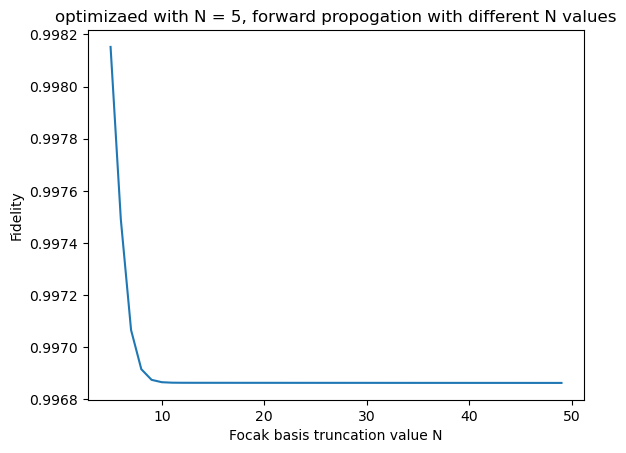
\includegraphics[width=0.6\linewidth]{vac2coherent_N_convergence.png}
    \caption{cavity state Fock basis truncation $N$ convergence}
    \label{fig:vac2coherent_N_convergence}
\end{figure}

\begin{figure}[H]
    \centering
    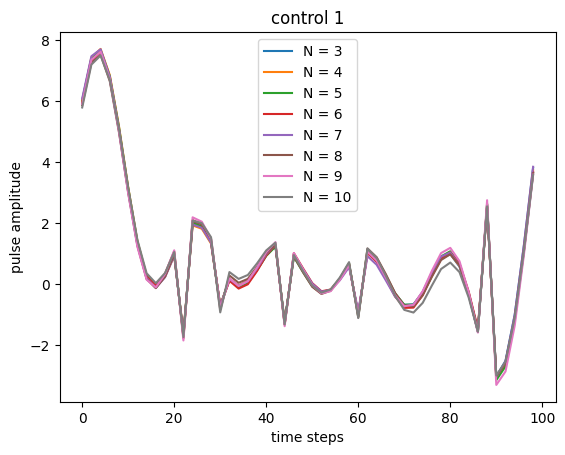
\includegraphics[width=0.6\linewidth]{check_convergence_control1.png}
    \caption{cavity state Fock basis truncation $N$ convergence}
    \label{fig:check_convergence_control1}
\end{figure}

\begin{figure}[H]
    \centering
    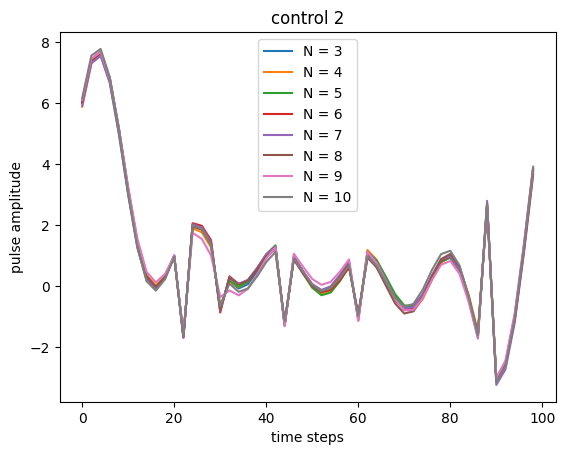
\includegraphics[width=0.6\linewidth]{check_convergence_control2.png}
    \caption{cavity state Fock basis truncation $N$ convergence}
    \label{fig:check_convergence_control2}
\end{figure}

%%%%%%%%%%%%%%%%%%%%%%%%%%%%%%%
\subsection{Diagnostic pulse: unselective spin flip, cavity coupled with single qubit(effective)}
Going from a cavity cavuum state to a cavity coherent state analytically requires only a displacement operation
which requires only a control pulse to the cavity. Hence, in the previous disagnostic scenario the full Hamiltonia
with all three (real) control channels were not used. 
\\
Here we consider the full system Hamiltonian (cavity + auxiliary qubit + coupling terms)
drift Hamiltoinan is given by, 
\begin{equation}
    H_d = \text{wr} * n_{\text{cavity}} + \text{Ez} * \sigma_z + \text{chi} * \sigma_z * (n_{\text{cavity}} + 1/2 )    
\end{equation}
where parameters of the physical system are:
\\
(notet that energy terms have unit $GHz$ and time terms have unit $ns$)
% TODO: ask chiyuan how to get these numbers
\begin{itemize}
    \item cavity frequency, wr = $2 \pi$
    \item qubit anharmonicity Ez = $0.44 \pi$
    \item qubit-cavity coupling strength chi = $0.007$
\end{itemize}

Real control channels in the Hamiltonain are given by (each term comprises a channel): 
\begin{equation}
    H_c = a + a^{\dagger} + -1j*(a - a^{\dagger}) + \sigma_x    
\end{equation}

The initial and target states for this pulse optimization code are: 
\begin{align*}
    \psi_0 &= \frac{1}{\sqrt{2}} (\ket{0}_{\text{cavity}} \otimes \ket{0}_{\text{qubit}} 
                + \ket{1}_{\text{cavity}} \otimes \ket{0}_{\text{qubit}})\\
    \psi_{\text{targ}} &= \frac{1}{\sqrt{2}} (\ket{0}_{\text{cavity}} \otimes \ket{1}_{\text{qubit}} 
                + \ket{1}_{\text{cavity}} \otimes \ket{1}_{\text{qubit}})\\
\end{align*}

where the qubit state is flipped irrepsective of the cavity state
\\
The final optimization algorithm parameters are:
\\ 
%TODO: ask chiyuan how the appropriate pulse length is calcualted
\begin{itemize}
    \item optimization algorithm: GRAPE
    \item Number of time slots, n\_ts = 500
    \item Time allowed for the evolution, evo\_time = 1
    \item Fidelity error target, fid\_err\_targ = 1e-3
    \item Maximum iterations for the optisation algorithm, max\_iter = 1000
    \item Maximum (elapsed) time allowed in seconds, max\_wall\_time = 120
    \item initial guess pulse type, p\_type = 'LIN'
\end{itemize}

The inital and optimized pulses are: 
\begin{figure}[H]
    \centering
    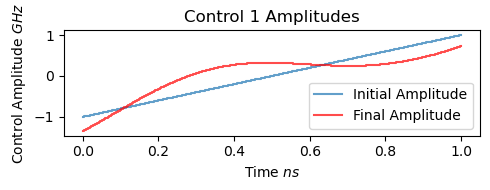
\includegraphics[width=0.6\linewidth]{unselective_spin_flip_control1.png}
    \caption{unselective spin flip control 1 pulse amplitudes}
    \label{fig:unselective_spin_flip_control1}
\end{figure}
\begin{figure}[H]
    \centering
    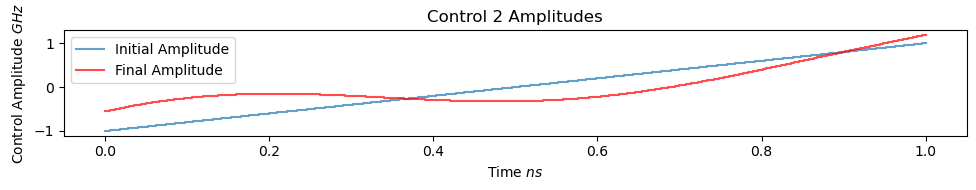
\includegraphics[width=0.6\linewidth]{unselective_spin_flip_control2.png}
    \caption{unselective spin flip control 2 pulse amplitudes}
    \label{fig:unselective_spin_flip_control2}
\end{figure}
\begin{figure}[H]
    \centering
    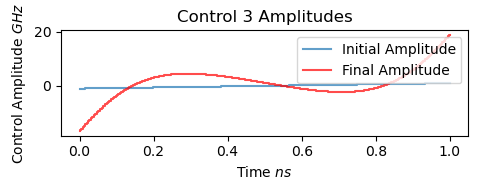
\includegraphics[width=0.6\linewidth]{unselective_spin_flip_control3.png}
    \caption{unselective spin flip control 3 pulse amplitudes}
    \label{fig:unselective_spin_flip_control3}
\end{figure}

Forward simulation is given below to ensure that pulse optimization has run properly. 
\\
Simulation gives: 
\begin{itemize}
    \item sesolve final fidelity:  0.9995869703894827
    \item self-implemented final fidelity:  0.9995575205270999
\end{itemize}
\begin{figure}[H]
    \centering
    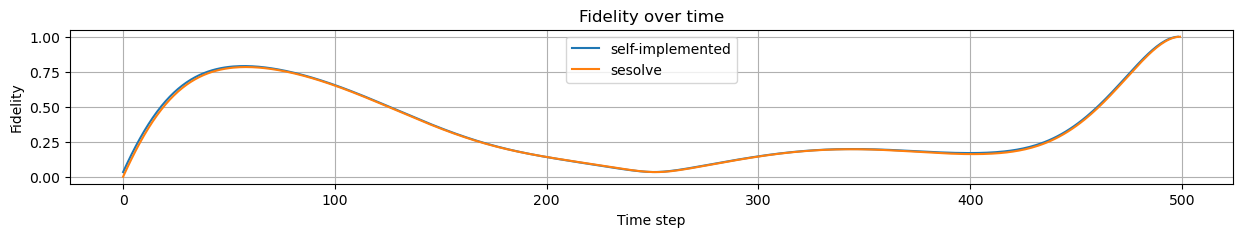
\includegraphics[width=0.6\linewidth]{unselective_spin_flip_simulation.png}
    \caption{unselective spin flip forward simulation}
    \label{fig:unselective_spin_flip_forward_simulation}
\end{figure}

%%%%%%%%%%%%%%%%%%%%%%%%%%%%%%%
\subsection{Diagnostic pulse: selective spin flip, cavity coupled with single qubit(effective)}

For this scenario, the drift and contorl Hamiltonian terms are same as in the previous section. We are interested in this state 
preparation because as achieved by Krastanov et al.(2015) \cite{Krastanov2015} which gave a contruction for how to achieve arbitrary 
operation on dispersively coupled cQED systems using a set of two opeartions: displacements and selective number-dependent arbitrary phase (SNAP) operations. 
SNAP operations allow an arbitrary set of relative phases to be applied to different photon number states, and can be represented with the form
\begin{equation}
    S(\vec{\theta}) = \sum_k e^{i\theta_k} \ket{k}\bra{k}
\end{equation}

Clearly, SNAP operations require selective spin rotations of which selective spin flip is a special case.
\\
State preparation optimization target is as follow: 
\begin{align*}
    \psi_0 &= \frac{1}{\sqrt{2}} (\ket{0}_{\text{cavity}} \otimes \ket{0}_{\text{qubit}} 
                + \ket{1}_{\text{cavity}} \otimes \ket{0}_{\text{qubit}})\\
    \psi_{\text{targ}} &= \frac{1}{\sqrt{2}} (\ket{0}_{\text{cavity}} \otimes \ket{0}_{\text{qubit}} 
                + \ket{1}_{\text{cavity}} \otimes \ket{1}_{\text{qubit}})\\
\end{align*}
(where qubit spin flip is selective on cavity state)
% TODO: 问chiyuan,selective spin flip 和 unselective spin flip 的主要区别在哪
% discuss 
% - selective spin flip 和 unselective spin flip 的主要区别在哪
% - why is selective spin flip the next step
% - discuss pulse amplitude constraint
% - ask chiyuan how the appropriate pulse length is calcualted
% - figure out about the cavity state going to higher photon number state inbetween state transition

\\

The best optimization result that was obtained by tuning the optimization script from 
previous section is as follow. 
\\
The final optimization algorithm parameters are:
\\ 
\begin{itemize}
    \item optimization algorithm: GRAPE
    \item Number of time slots, n\_ts = 100000
    \item Time allowed for the evolution, evo\_time = 500
    \item Fidelity error target, fid\_err\_targ = 1e-8
    \item Maximum iterations for the optisation algorithm, max\_iter = 10000
    \item Maximum (elapsed) time allowed in seconds, max\_wall\_time = 7200
    \item initial guess pulse type, p\_type = 'SINE'
\end{itemize}

The inital and optimized pulses are: 
\begin{figure}[H]
    \centering
    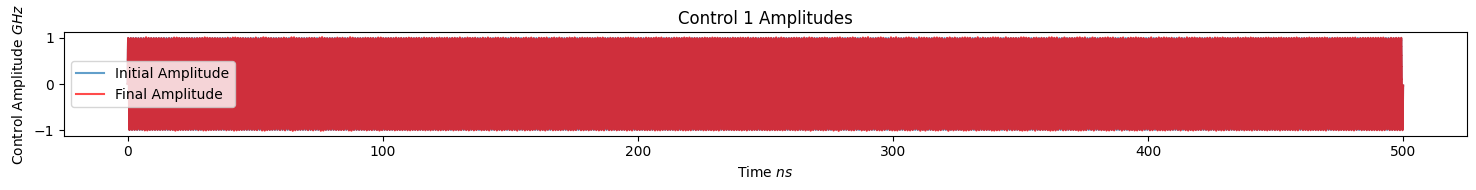
\includegraphics[width=0.6\linewidth]{selective_spin_flip_GRAPE_control1.png}
    \caption{selective spin flip control 1 pulse amplitudes}
    \label{fig:selective_spin_flip_control1}
\end{figure}
\begin{figure}[H]
    \centering
    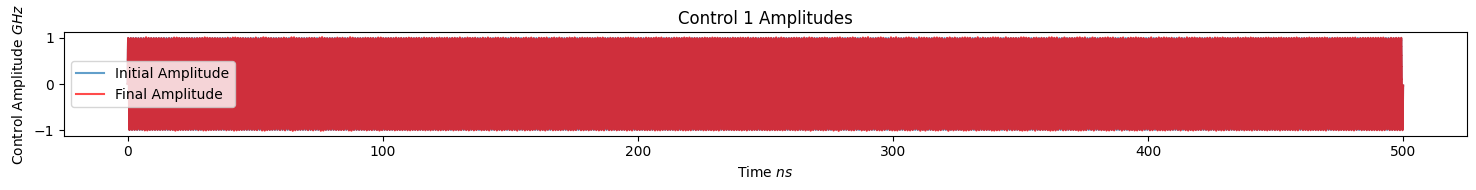
\includegraphics[width=0.6\linewidth]{selective_spin_flip_GRAPE_control1.png}
    \caption{selective spin flip control 2 pulse amplitudes}
    \label{fig:selective_spin_flip_control2}
\end{figure}
\begin{figure}[H]
    \centering
    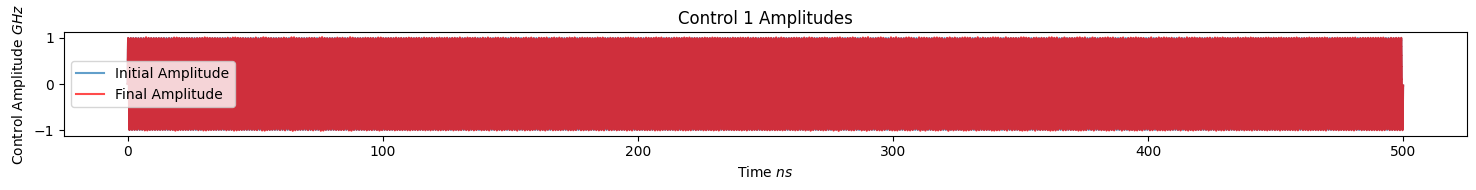
\includegraphics[width=0.6\linewidth]{selective_spin_flip_GRAPE_control1.png}
    \caption{selective spin flip control 3 pulse amplitudes}
    \label{fig:selective_spin_flip_control3}
\end{figure}

The control pulses have very fast oscillations due to the large number of time slices.
Zooming into control 1 pulse amplitudes, as shown in fig \ref{fig:selective_spin_flip_control3_zoomin},
we see that the pulse is fairly smooth. However, this fast oscillation is still not desirable and preferably gotten rid of. 
Another reason that might have contributed to this fast oscillation is the background frequency of the cavity and qubit 
of which the control pulses are trying to cancel out. One way to partially deal with this fast oscillation issue is to work
with the Hamiltonian in the rotating frame which will be tried out in the next section when cavity vacuum state to cavity cat state
is being optimized. 

\begin{figure}[H]
    \centering
    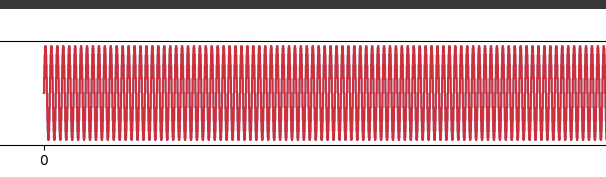
\includegraphics[width=0.6\linewidth]{selective_spin_flip_GRAPE_control1_zoomin.png}
    \caption{selective spin flip control 1 pulse amplitudes zoomed in}
    \label{fig:selective_spin_flip_control3_zoomin}
\end{figure}

Forward simulation is given below to ensure that pulse optimization has run properly. 
\\
Simulation gives: 
\begin{itemize}
    \item sesolve final fidelity:  0.9994876128337873
    \item cavity ptrace fidelity:  0.9997184822307845
    \item qubit ptrace fidelity:  0.999999719275808
    \item self-implemented final fidelity:  0.9997005493228243
\end{itemize}
\begin{figure}[H]
    \centering
    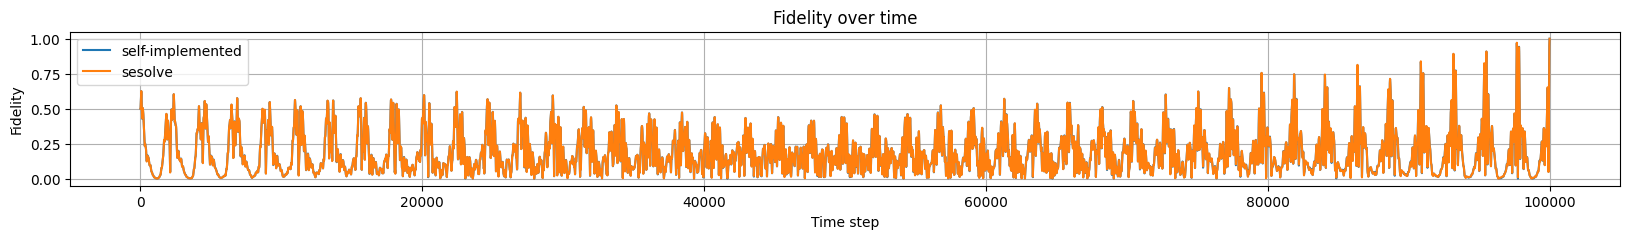
\includegraphics[width=0.6\linewidth]{selective_spin_flip_GRAPE_simulation.png}
    \caption{selective spin flip forward simulation}
    \label{fig:selective_spin_flip_forward_simulation}
\end{figure}


A particular analytical solution as given by Chiyuan already gives fidelity of $~0.98$.
            We expect a higher fidelity from a numerical optimization solution. 
            % TODO: ask chiyuan for analytical solution and put here
\\
However, this numerical solution has the folowing issues.
The optimzied pulses go beyong the amplitude constrains that required for the effective Hamiltonian to be valid. 
When the pulse amplitdes constrained are supplied to the optimziation algorithms, the results are not very satisfactory. 
% TODO: try the code with pulse amplitude constraints}

\\

The following run has two modifications: 
\begin{itemize}
    \item initial guess pulse is changed from sindusoidal to linear to see whether this improves the fast oscillation issue
    \item Pulse amplitude constraints are added to the optimization algorithm
\end{itemize}
However, as can be seen from the optimized pulses below, the fast oscillation issue is not resolved well. 
This is especially so for control 3.
\\

The inital and optimized pulses are: 
\begin{figure}[H]
    \centering
    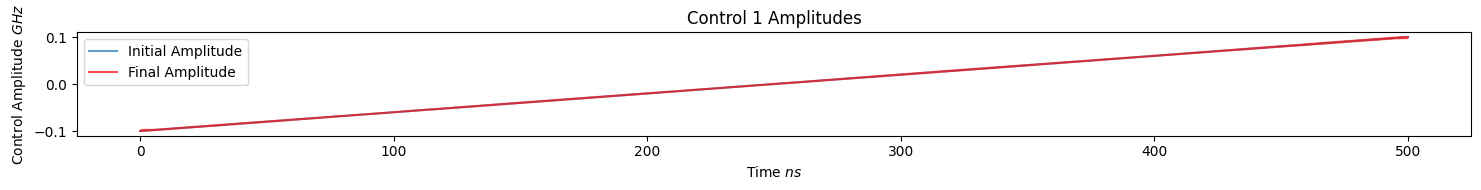
\includegraphics[width=0.6\linewidth]{selective_spin_flip_GRAPE_500,_100_000_LIN_constraints_control1.png}
    \caption{selective spin flip control 1 pulse amplitudes}
    \label{fig:selective_spin_flip_constrains_control1}
\end{figure}
\begin{figure}[H]
    \centering
    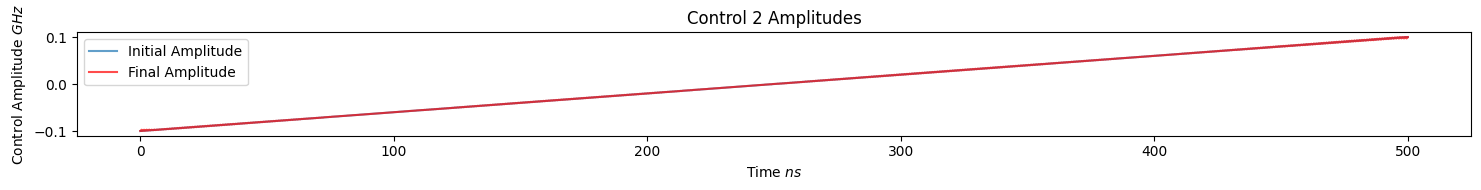
\includegraphics[width=0.6\linewidth]{selective_spin_flip_GRAPE_500,_100_000_LIN_constraints_control2.png}
    \caption{selective spin flip control 2 pulse amplitudes}
    \label{fig:selective_spin_flip_constrains_control2}
\end{figure}
\begin{figure}[H]
    \centering
    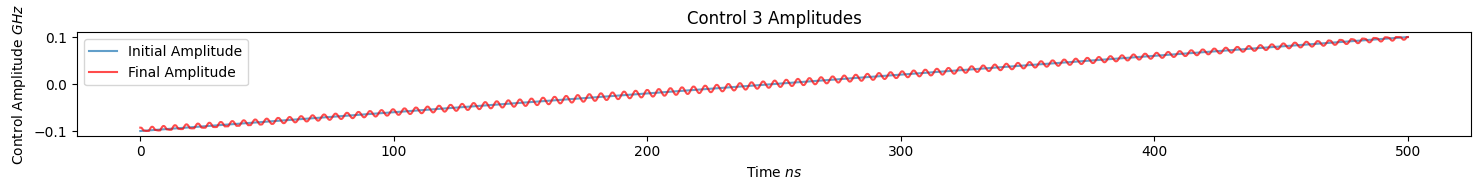
\includegraphics[width=0.6\linewidth]{selective_spin_flip_GRAPE_500,_100_000_LIN_constraints_control3.png}
    \caption{selective spin flip control 3 pulse amplitudes}
    \label{fig:selective_spin_flip_constrains_control3}
\end{figure}

Forward simulation is given below to ensure that pulse optimization has run properly. 
\\
Simulation gives: 
\begin{itemize}
    \item sesolve final fidelity:  0.9992259750482354
    \item cavity ptrace fidelity:  0.9992525011412332
    \item qubit ptrace fidelity:  0.9992706948956261
    \item self-implemented final fidelity:  0.9999937323329505
\end{itemize}
\begin{figure}[H]
    \centering
    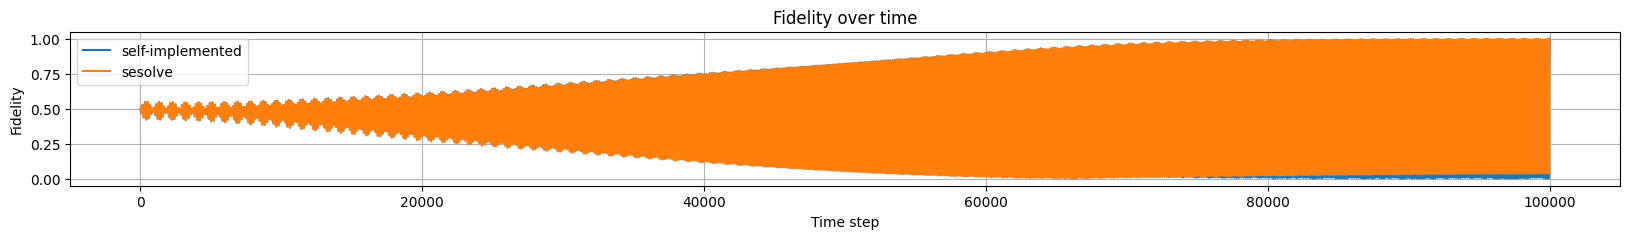
\includegraphics[width=0.6\linewidth]{selective_spin_flip_GRAPE_500,_100_000_LIN_constraints_simulation.png}
    \caption{selective spin flip forward simulation}
    \label{fig:selective_spin_flip_constraints_forward_simulation}
\end{figure}

At this point, we continued varying the parameters (puse length, number of slices, initial guess pulse, etc.). 
However, none gave optimization results where fidelity, pulse amplitude, pulse smoothness and fast oscillation issue 
are all accounted for satisfactorily. 

%%%%%%%%%%%%%%%%%%%%%%%%%%%%%%%
\subsection{vacuum to cat state, cavity coupled with single qubit(effective)}
In this section, we finally get to do a state preparation optimization of cavity vacuum state to cavity cat state.
The most efficient way to do this is to optimize for the cavity state alone by tracing out the qubit state when calculating state fidelity. 
However, the QuTip package does not support this feature. I attemped to modify QuTip source code to allow for this feature but failed. 
One might naively think that QuTip calculates state fidelity at the end of each optimization iteration. 
Intead, QuTip calculates the state fidelity throughout the entire control pulse evolution for some caching purposes that improves the overall performance of the optimization algorithm. 
Here, a problem arises as tracing out qubit state in the middle of a pulse is not valid. 
% WHY? 
\\
Hence, composite state of the cavity and qubit was still used for optimization which restricts the search space to smaller than ideal. 
However, the optimization results as shown below were not very satisfacotry. 
\\
The final optimization algorithm parameters are:
\\ 
%TODO: ask chiyuan how the appropriate pulse length is calcualted
\begin{itemize}
    \item optimization algorithm: GRAPE
    \item Number of time slots, n\_ts = 100000
    \item Time allowed for the evolution, evo\_time = 5000
    \item Fidelity error target, fid\_err\_targ = 1e-8
    \item Maximum iterations for the optimization algorithm, max\_iter = 10000
    \item Maximum (elapsed) time allowed in seconds, max\_wall\_time = 21600
    \item initial guess pulse type, p\_type = 'SIN'
\end{itemize}
% TODO: show estimation of pulse length

The inital and optimized pulses are: 
\begin{figure}[H]
    \centering
    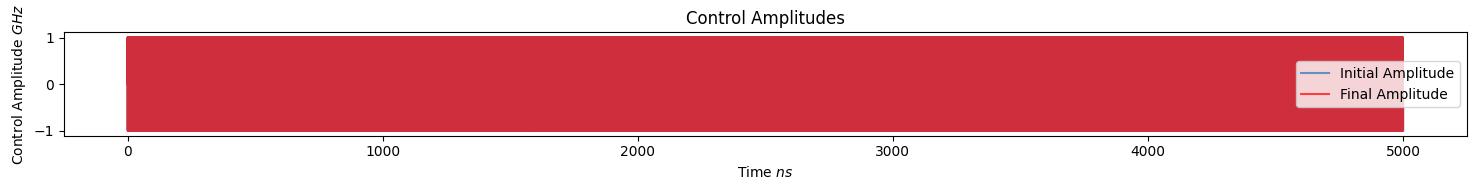
\includegraphics[width=0.6\linewidth]{vac2cat_effective_Hamiltonian_GRAPE_control1.png}
    \caption{vacuum to cat state control 1 pulse amplitudes}
    \label{fig:vac2cat_effective_Hamiltonian_GRAPE_control1}
\end{figure}
\begin{figure}[H]
    \centering
    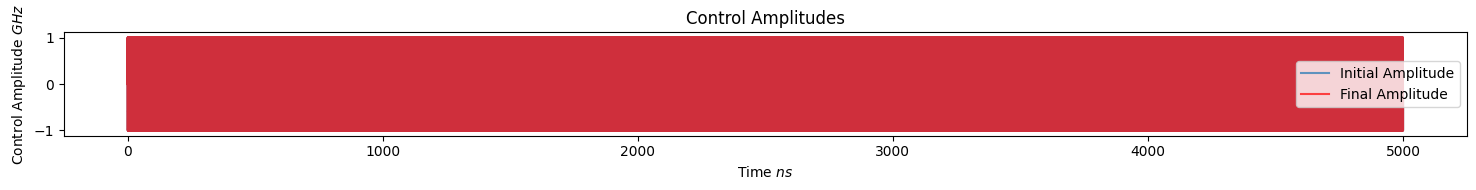
\includegraphics[width=0.6\linewidth]{vac2cat_effective_Hamiltonian_GRAPE_control2.png}
    \caption{vacuum to cat state control 2 pulse amplitudes}
    \label{fig:vac2cat_effective_Hamiltonian_GRAPE_control2}
\end{figure}
\begin{figure}[H]
    \centering
    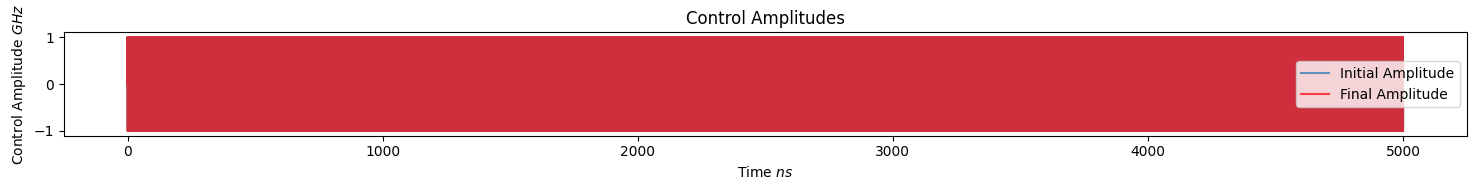
\includegraphics[width=0.6\linewidth]{vac2cat_effective_Hamiltonian_GRAPE_control3.png}
    \caption{vacuum to cat state control 3 pulse amplitudes}
    \label{fig:vac2cat_effective_Hamiltonian_GRAPE_control3}
\end{figure}

Forward simulation is given below to ensure that pulse optimization has run properly. 
\\
Simulation gives: 
\begin{itemize}
    \item sesolve final fidelity:  0.4390558062780975
    \item cavity ptrace fidelity:  0.44320315443027297
    \item qubit ptrace fidelity:  0.9871678390509413
    \item self-implemented final fidelity:  0.9529111010142354
\end{itemize}
\begin{figure}[H]
    \centering
    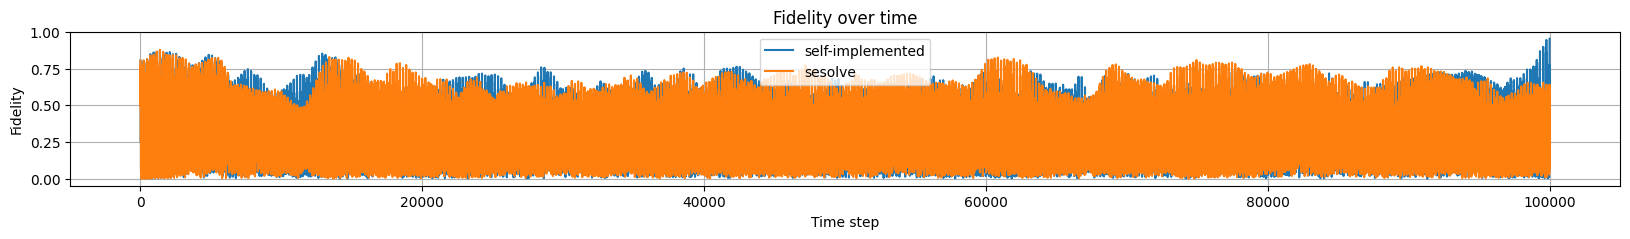
\includegraphics[width=0.6\linewidth]{vac2cat_effective_Hamiltonian_GRAPE_simulations.png}
    \caption{vacuum to cat state forward simulation}
    \label{fig:vac2cat_effective_Hamiltonian_GRAPE_simulations}
\end{figure}

It can be seen that the optimization results are not very satisfactory. 
Many tunings were attempted but none gave satisfactory results.
\\
At this point, we turned to look at a new python quantum control optimziation library, Krotov which builds on top of QuTip,
to see whether it can give better optimization results. Krotov’s optimization method is a gradient-based optimization algorithm like GRAPE. 
Krotov’s method distinguishes itself by guaranteeing monotonic convergence for near-continuous control fields. 
Besides the difference in optimization algorithm used, the Krotov package has the following incentives to be tried: 
\begin{itemize}
    \item Krotov is much better implemented than QuTip. For instance, Krotov allows display of optimization progress for every iteration. 
    \item Krotov allows inbuilds better customizability than QuTip. 
            For instance, Krotov allows for the optimization of the fidelity to be optimized.
\end{itemize}

Besides switching from QuTip to Krotov, the Hamiltonians are also redefined to be an interaction picture. 
The drift Hamiltonian ($H_0$) and control Hamiltonians ($H_1$, $H_2$, $H_3$) are defined as follows:

1. \textbf{Drift Hamiltonian} ($H_0$):
\begin{equation}
H_0 = \hbar \omega_r a^\dagger a + \frac{E_s}{2} \sigma_z + \frac{E_m}{2} \tau_z - \chi_m \tau_z \left(a^\dagger a + \frac{1}{2}\right) - \chi_s \sigma_z \left(a^\dagger a + \frac{1}{2}\right) - \frac{\chi_0}{2} \sigma_z \tau_z,
\end{equation}
where $\omega_r$ is the resonator frequency, $a$ and $a^\dagger$ are the annihilation and creation operators of the cavity, $E_s$ and $E_m$ are the energy levels of the qubit and the molecular orbital, $\sigma_z$ and $\tau_z$ are the Pauli Z operators for the qubit and the molecular orbital, respectively, and $\chi_m$, $\chi_s$, and $\chi_0$ are the dispersive shifts.

2. \textbf{Control Hamiltonians}:
   - $H_1$: This control Hamiltonian corresponds to the real part of the cavity drive. It is given by
     \begin{equation}
     H_1 = \left(a + a^\dagger\right),
     \end{equation}
     where $a$ and $a^\dagger$ are the annihilation and creation operators of the cavity.

   - $H_2$: This control Hamiltonian corresponds to the imaginary part of the cavity drive. It is given by
     \begin{equation}
     H_2 = -i\left(a - a^\dagger\right),
     \end{equation}
     where $a$ and $a^\dagger$ are the annihilation and creation operators of the cavity.

   - $H_3$: This control Hamiltonian corresponds to the drive on the qubit. It is given by
     \begin{equation}
     H_3 = \sigma_x,
     \end{equation}
     where $\sigma_x$ is the Pauli X operator for the qubit.
\\
The optimized results are as follow. 
\begin{figure}[H]
    \centering
    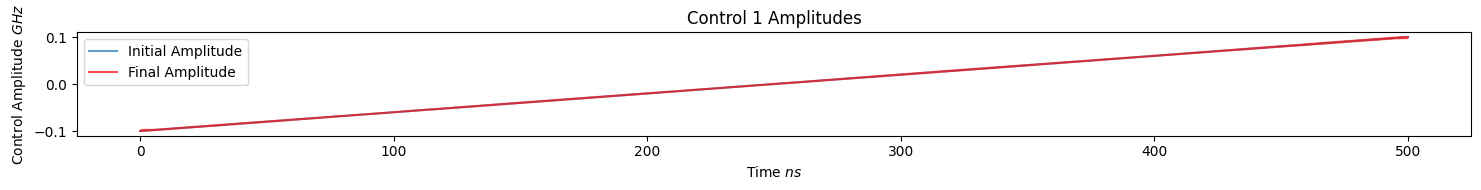
\includegraphics[width=0.6\linewidth]{selective_spin_flip_GRAPE_500,_100_000_LIN_constraints_control1.png}
    \caption{selective spin flip control 1 pulse amplitudes}
    \label{fig:selective_spin_flip_constrains_control1}
\end{figure}
\begin{figure}[H]
    \centering
    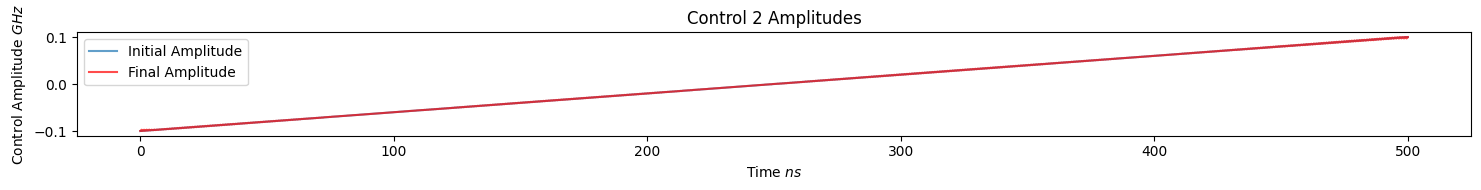
\includegraphics[width=0.6\linewidth]{selective_spin_flip_GRAPE_500,_100_000_LIN_constraints_control2.png}
    \caption{selective spin flip control 2 pulse amplitudes}
    \label{fig:selective_spin_flip_constrains_control2}
\end{figure}
\begin{figure}[H]
    \centering
    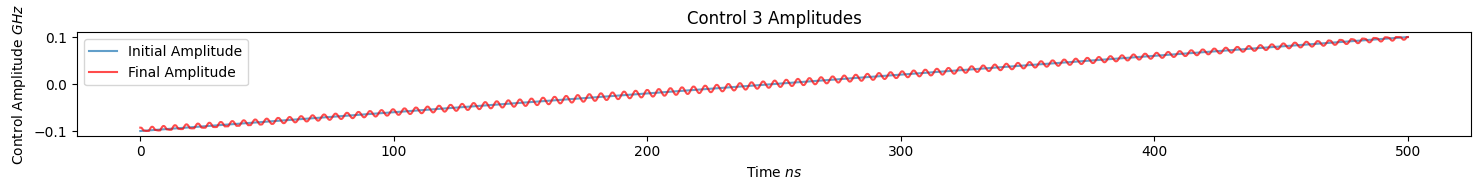
\includegraphics[width=0.6\linewidth]{selective_spin_flip_GRAPE_500,_100_000_LIN_constraints_control3.png}
    \caption{selective spin flip control 3 pulse amplitudes}
    \label{fig:selective_spin_flip_constrains_control3}
\end{figure}

Forward simulation is given below to ensure that pulse optimization has run properly. 
\\
Simulation gives: 
\begin{itemize}
    \item sesolve final fidelity:  0.9992259750482354
    \item cavity ptrace fidelity:  0.9992525011412332
    \item qubit ptrace fidelity:  0.9992706948956261
    \item self-implemented final fidelity:  0.9999937323329505
\end{itemize}
\begin{figure}[H]
    \centering
    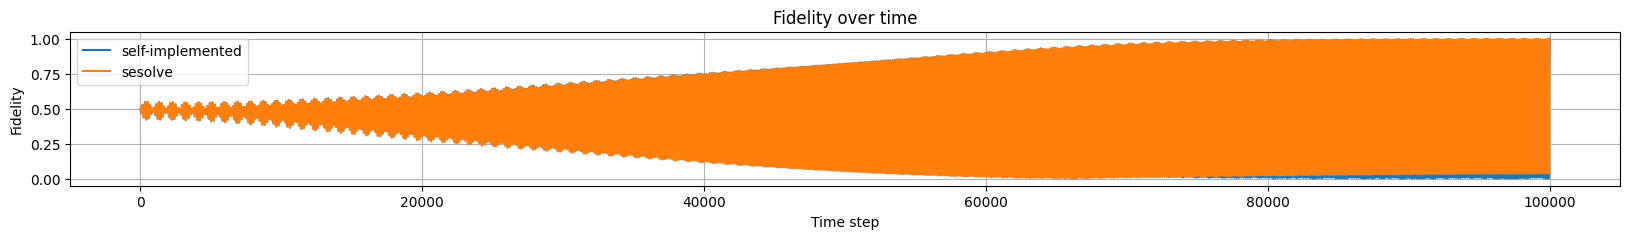
\includegraphics[width=0.6\linewidth]{selective_spin_flip_GRAPE_500,_100_000_LIN_constraints_simulation.png}
    \caption{selective spin flip forward simulation}
    \label{fig:selective_spin_flip_constraints_forward_simulation}
\end{figure}



%%%%%%%%%%%%%%%%%%%%%%%%%%%%%%%
\subsection{Further discussions reagarding numerical pulse optimzation}
\begin{enumerate}
    \item choosing time parameters: 
        \begin{itemize}
            \item evolution time (evo\_time): pulse length needed can be estimated %TODO: ask chiyuan how is this calculated
            \item number of time slices (n\_ts): n\_ts that is too small will lead to large error; 
                n\_ts that is too large will result in long computation time; 
                hence an appropriate n\_ts value needs to be tested via trial and error.
        \end{itemize}
    \item 
\end{enumerate}

%%%%%%%%%%%%%%%%%%%%%%%%%%%%%%%%%%%%%%%%%%%%%%%%%%%%%%%%%%%%%%%
\section{Physical realizability}
go back the Hamiltonian massagiing: Perturbation, frame change, throwing away small cross terms, exact \\
compare fidelity

\section{Future work}

\section{Conclusion}


\printbibliography
\end{document}